%=============================================================================
% Thesis Template in LaTex
%
% File:  1-Introduction.tex -- Introduction to the topic
% Author(s): Jürgen Hackl <hackl@ibi.baug.ethz.ch>
%            Clemens Kielhauser <kielhauser@ibi.baug.ethz.ch>
%
% Creation:  27 Jan 2014
% Time-stamp: <Tue 2013-08-13 20:14 juergen>
%
% Copyright (c) 2014 Infrastructure Management Group (IMG)
%               http://ibi.ethz.ch
%
% More information on LaTeX: http://www.latex-project.org/
%=============================================================================

\chapter{Einleitung}
\label{chap:Einleitung}

\section{Some formal aspects}
\label{sec:formalaspects}

Strong demands can only be met with the help of a very stringent and clear structure laid out at the beginning of the writing process. One of the most clear structuring is given by a rigorous "legal numbering" (1, 1.1, 1.1.1 etc.). It is good to know that \LaTeX does all this formatting business without any need to renumber things yourself at each iteration and so on. Thus we strongly recommend using \LaTeX for the project. Anything else (e.g. Word) is a mess when writing an elaborate scientific text with many graphics and formulas.

Even a particular elusive reader should be able to quickly glean the most important thoughts, experiments and results from just looking at illustrative schematics, diagrams, and pictures with self explaining, extensive figure captions.

There are always parts/chapters/sections of text which are complex and important for a full description and documentation of the work, but not absolutely necessary for following the main lines of thought. It is very helpful for the somewhat more interested, but temporally limited reader if such passages of text are correspondingly marked, e.g. by a brief introductory remark to such sections, or even by moving them into appendices.

Definitively each chapter and ideally also each section should begin with a short guide: what is communicated in the following text, which sources (quote clearly) have been used, what are the basic concepts used and which goals are to be reached. Similarly, at the end of larger elaborations a short synopsis of the communicated content should be
offered.

\subsection{Plain text}
\label{sec:plaintext}

A single font must be used throughout the thesis or report, the only exceptions being in tables, graphs, and appendices. Headings may be bolded and no more than 2 points larger than the rest of the text.

The page format should be single column with one and a single spacing used
between the lines. Spacing of words on a line should be such that the line can be easily read. Crowding words together or leaving excessive spaces is not permitted.

\subsection{Footnotes}
\label{sec:footnotes}


For those who are using footnotes\footnote{Some example footnote.}, Arabic numerals are used consecutively throughout a chapter, and should normally appear at the bottom of the relevant page, keyed to the same number following the word or phrase in the text to which it refers. If a footnote is too long for the relevant page, it may be continued on the following page preceding the footnotes for that page. If the number of footnotes is very large, numbers may be restarted with each chapter.


\subsection{Lists}
\label{sec:lists}

There are three types of lists with the environment names \emph{itemize}, \emph{enumerate} and \emph{description}. All lists have a separation between each item, to improve the reading of item texts spanning several lines. This item text can contain multiple paragraphs. These paragraphs are appropriately spaced and indented according to their position in the list. 

\begin{itemize}
\item 
The \emph{itemize} sets off list items with \emph{bullets}, like this.
%
\item Of course, lists can be nested, each type up to at least four levels.
One type of list can be nested within another type.
%
  \begin{itemize}
  \item Nested lists of the same type will change style of numbering 
  or \emph{bullets} as needed.
  \end{itemize}
\end{itemize}
%
\begin{enumerate}
\item The \emph{enumerate} environment numbers the list elements.

This is a new paragraph in the item text, which is not intended as in the normal text but separated from the previous paragraph.
%
\item The enumeration scheme changes with each nesting level
  \begin{enumerate}
  \item as shown in this nested enumerated list item.
  \end{enumerate}
\end{enumerate} 

\begin{description}
\item[Some description] The \emph{description} environment allows to describe some content.
\end{description}

\subsection{Mathematical symbols and equations}
\label{sec:math}

Each formula, except for generally accepted and well-known formulas, either has to be mathematically derived, to be explained, or a literature source has to be provided. This applies especially to complex models, where each constraint should be described and explained.

There are three types of mathematical equations: (a) in-line equations, (b) displayed butunnumbered equations, and (c) displayed and numbered equations.

\subsubsection{In-line equations}
\label{sec:inlineeq}

An in-line equation is used for particularly simple relationships which (i) do not need vertical space for integrals, fractions, etc., (ii) can be expressed without breaking the flow of the sentence, and (iii) will not be referenced again in the document.

For example:

\begin{IMleftrightskip}
If volume $V$ and temperature $T$ are known, the ideal gas law can be used to get a reasonable approximation for the pressure of a gas as $P=nRT/V$, where $n$ is the number of moles of gas and $R$ is the gas constant.
\end{IMleftrightskip}

Unless all the variables have been defined earlier in the document, the physical significance of all the quantitie s appearing in an equation must be stated at the point of their first appearance in the document.

\subsubsection{Displayed, but unnumbered, equations}
\label{sec:diuneq}

Equations that are too complex to be written as in-line equations should be "displayed", which usually means, that the equation is centered between the left and right margins or aligned at a tab stop
with some indent from the left margin and some vertical space is provided above and below the equation to set it apart from the text.

For example:


\begin{IMleftrightskip}
The van der Waals equation is used to provide a more accurate expression for the pressure $P$ as a function of the molar volume $V_m$ and the temperature $T$ as
%
\begin{equation*}
P = \frac{RT}{V_m-b}-\frac{a}{V_m^2}~,
\end{equation*}
%
where $a$ and $b$ are van der Waals parameters for the gas.

or

The electric field $\mathbf{E}$ at the origin due to a point charge $q$ at a distance $r$ is given by
%
\begin{equation*}
\mathbf{E} = \frac{|q|}{4\pi\varepsilon_0 r^2}\mathbf{\hat{r}}
\end{equation*}
where $\mathbf{\hat{r}}$ is the position vector of the point charge.
\end{IMleftrightskip}

Note that in the examples presented above, the displayed equation is part of the text, i.e, it is punctuated, and incorporated in to the structure of the sentence.

All the scalar variables are italicized whereas the vector quantities in the second example are Roman boldfaced.

\subsubsection{Displayed and numbered equations}
\label{sec:dineq}

One often has to refer back to the important equations. The standard way to do this is by referring to the equation number. Of course, in order to refer to an equation number, one must first number the equations. A consiste nt system of numberi ng equations must be adopted. Various options are:
\begin{itemize}
\item Number equations as (1), (2), etc., starting in Chapter 1 (or at the first numbered equation) and continuing until the end of the last numbered equation in the document.
\item Incorporate the chapter number into the equation, as in (1.1),  (2.3), (4.6), etc., which means the equation numbering goes back to 1 at the beginning of each chapter.
\item Use Roman numerals for chapter numbers, as in (I.1), (II.3), (IV.6) etc.
\end{itemize}

For example:

\begin{IMleftrightskip}
The non-relativistic Schrödinger equation for a particle of mass m
subject to a potential energy function V(x) in a one-dimensional universe is
%
\begin{equation}
  \label{eq:1}
  E \psi(x) = \frac{-\hbar^2}{2m} \frac{d^2\psi}{d x^2} + V(x)\psi(x)
\end{equation}
%
where $\hbar = h/(2\pi)$, $h$ is Plack’s constant, and $E$ is the total energy of the system.
\end{IMleftrightskip}

The equation in the example is approximately centered on the page, and the equation number is aligned by a right-tab at the right margin.

To cite an equation in text, use an abbreviation if it is not the first word of the sentence. Suitable singular and plural ab breviations include eq. and eqs., Eq. and Eqs. Spell out “Equation” when it is the first word of a sentence and when it is not accompanied by a number.

The used numbering of the equation may change according to the context of the work. E.g. number them as subequations
\begin{subequations}
\begin{align}
  \dot{q}_i & = \frac{\partial H}{\partial p_i} \\
  \dot{p}_i & = -\frac{\partial H}{\partial q_i} 
\end{align}
\end{subequations}
or with only a single number
\begin{equation}
\begin{aligned}
  \dot{q}_i & = \frac{\partial H}{\partial p_i} \\
  \dot{p}_i & = -\frac{\partial H}{\partial q_i} 
\end{aligned}
\end{equation}
Many further possibilities of displaying equations exist.

%\subsection{Theorems}
%\label{sec:theorems}

\subsection{Tables}
\label{sec:tables}

Tables should only be used to present three (3) or more items; otherwise, the data should be described in the narrative. Tables should be arranged so like material appears in columns, not rows. Information presented in tables should be sufficiently understandable so frequent reference to the narrative is unnecessary. Each table should have a title, generally appearing above the table itself. The table title and other items may be footnoted, although extensive explanations appearing in footnotes should be avoided. All abbreviations and symbols should be defined.

Tables are generally no more than what can be printed on one page, but occasionally multi-paged tables are necessary and are acceptable. Tables may appear on pages which contain narrative text or tables may appear singularly on a page (i.e. one table per page and only the table on the page).

%=============================================================================
% Thesis Template in LaTex
%
% File:  t-05-01-IsingModel.tex -- Table for the Ising
% Author(s): Juergen Hackl <hackl@ibi.baug.ethz.ch>
%            Clemens Kielhauser <kielhauser@ibi.baug.ethz.ch>
%
% Creation:  27 Jan 2014
% Time-stamp: <Tue 2013-08-13 20:14 juergen>
%
% Copyright (c) 2014 Infrastructure Management Group (IMG)
%               http://ibi.ethz.ch
%
% More information on LaTeX: http://www.latex-project.org/
%=============================================================================

\begin{table}[ht]
\centering
\small\renewcommand{\arraystretch}{1.2}  
%
\captionabove[Mean-field predictions for the critical temperature of the Ising model]{Comparison of the mean-field predictions for the critical temperature of the Ising model with exact results and the best known estimates for different spatial dimensions $d$ and lattice symmetries.}
\label{tab:t-03-01-IsingModel}
%
\begin{tabularx}{0.5\textwidth}{lXXX}
\toprule
\textbf{lattice} & $d$ & $q$ & $T_\text{mf}/T_c$ \\
\hline
square  & 2 & 4 & 1.763 \\
%
triangular & 2 & 6 & 1.648 \\
%
diamond & 3 & 4 & 1.479 \\
%
simple cubic & 3 & 6 & 1.330 \\
%
bcc & 3 & 8 & 1.260 \\
%
fcc & 3 & 12 & 1.225 \\
\hline
\end{tabularx}
\end{table}

%=============================================================================
% EOF
%

%%% Local Variables:
%%% mode: latex
%%% TeX-master: "../guidelines"
%%% End:


\subsection{Figures}
\label{sec:figures}

Figures present charts, graphs, or images to the reader. Figure legends should be sufficiently detailed to allow the reader to understand without frequent reference to the narrative. However, overly detailed descriptions should be avoided. All abbreviations and symbols should be defined. Figure legends should appear on the same page and in the same orientation as the figure. For example, if the figure appears in landscape mode then the legend should also appear in landscape mode. If the figure legend is too lengthy to appear on the same page as the figure, then the legend, in its entirety, must appear on the next page.

Similar to tables, figures are usually constructed to be no more than what can appear on one page, but occasionally multi-paged figures are necessary. Figures may also appear singularly on pages or on pages containing narrative text.


\begin{figure}[h!]
  \centering
  %=============================================================================
% Thesis Template in LaTex
%
% File:  f-01-01-a-R-S.tex -- Classical Approach R-S
% Author(s): Jürgen Hackl <hackl@ibi.baug.ethz.ch>
%            Clemens Kielhauser <kielhauser@ibi.baug.ethz.ch>
%
% Creation:  27 Jan 2014
% Time-stamp: <Tue 2013-08-13 20:14 juergen>
%
% Copyright (c) 2014 Infrastructure Management Group (IMG)
%               http://ibi.ethz.ch
%
% More information on LaTeX: http://www.latex-project.org/
%=============================================================================

% ******
% Figure
% ******

% Document name
% =============

% f-00-00-a-Example.txt

% f  ... Figure
% 00 ... Chapter
% 00 ... Number of the figure
% a  ... Subfigure
% Ex ... Name of the figure


% Libraries
% =========

\usetikzlibrary{shapes,arrows}
\usetikzlibrary{positioning}
\usetikzlibrary{shadows}
\usetikzlibrary{backgrounds}
% \usepackage{verbatim}
\usetikzlibrary{automata}
\usetikzlibrary{arrows}
\usetikzlibrary{calc}
\usetikzlibrary{patterns}



% Styles
% ======

% Line Width
% ----------

\tikzstyle{hugeLine}=[line width=1.7pt]
\tikzstyle{bigLine}=[line width=1.3pt]
\tikzstyle{normalLine}=[line width=1pt]
\tikzstyle{smallLine}=[line width=.7pt]
\tikzstyle{tinyLine}=[line width=.5pt]

% Line Types
% ----------

\tikzstyle{Axis}=[smallLine,-to]
\tikzstyle{Line}=[normalLine]
\tikzstyle{Solid}=[fill=black!10]
\tikzstyle{Arrow}=[>=latex,smallLine,->]
\tikzstyle{Dimension}=[tinyLine,|-|]


% TikZ figure
% ===========

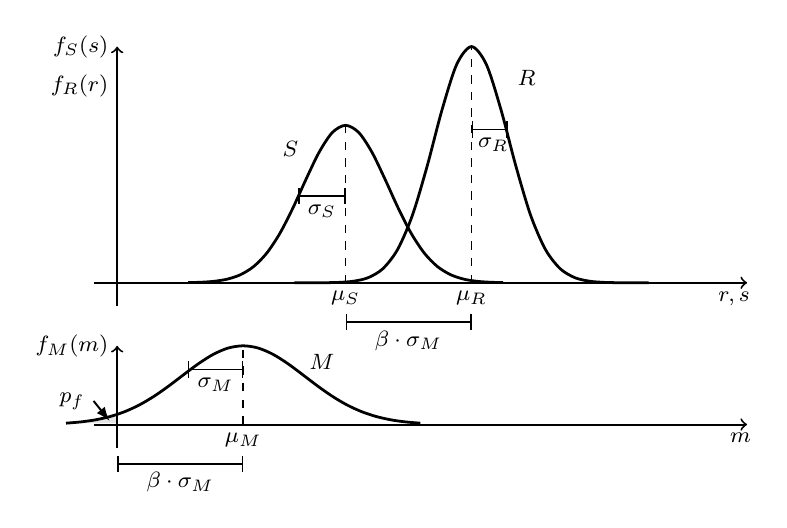
\begin{tikzpicture}


  % Grid
  % ----

  % \node [coordinate](ValA) at (0,0) {};
  % \node [coordinate](ValB) at (8,4) {};
  % \fill [fill=white](ValA) circle (.1pt);
  % \fill [fill=white](ValB) circle (.1pt);
  % \draw[help lines,step=1cm] (ValA) grid (ValB);

  \footnotesize

  % Distribution R
  \begin{scope}[xshift=4.5cm,yshift=0cm]
    \draw[tinyLine,dashed](0,0)--++(0,3) node [below,pos=0]{$\mu_R$};
    \draw[Dimension](0,1.95)--++(.46,0) node [below,pos=.6]{$\sigma_R$};
    \draw[Line,domain=-1.5:1.5,scale=1.5,smooth] plot (\x,{2*exp(-(\x)*(\x)*0.5/0.1)});
  \end{scope}

  \begin{scope}[xshift=2.9cm,yshift=0cm]
    \draw[tinyLine,dashed](0,0)--++(0,2) node [below,pos=0]{$\mu_S$};
    \draw[Dimension](0,1.1)--++(-.6,0) node [below,pos=.5]{$\sigma_S$};
  \draw[Line,domain=-2:2,scale=1,smooth] plot (\x,{2*exp(-(\x)*(\x)*0.5/0.3)});
  \end{scope}



  % \end{scope}

  % Axis
  \draw [Axis] (0,-.3)--(0,3) node [left, pos=1] {$f_S(s)$} node [left, pos=.85] {$f_R(r)$};
  \draw [Axis] (-.3,0)--(8,0) node [below, pos=.98] {$r,s$};

  % Comment
  \node (S) at (2.2,1.7){$S$};
  \node (R) at (5.2,2.6){$R$};
  \begin{scope}[xshift=0cm,yshift=-1.8cm]
  \begin{scope}[xshift=1.6cm,yshift=0cm]
    \fill[Solid,domain=-4.5:4.5,scale=.5,smooth] plot (\x,{2*exp(-(\x)*(\x)*0.5/2.5)});
    \fill[white](-1.6,0) rectangle (3.5,1);
    \draw[tinyLine,dashed](0,0)--++(0,1) node [below,pos=0]{$\mu_M$};
    \draw[Dimension](0,.7)--++(-.7,0) node [below,pos=.5]{$\sigma_M$};
    \draw[Line,domain=-4.5:4.5,scale=.5,smooth] plot (\x,{2*exp(-(\x)*(\x)*0.5/2.5)});
  \end{scope}

  % Dimension
  \draw[Dimension](0,-.5)--++(1.6,0) node [below,pos=.5]{$\beta\cdot \sigma_M$};

  % Arrow
  \draw [Arrow](-.3,.3)--(-.1,.05)node [left=0,pos=.0]{$p_f$};

  % Axis
  \draw [Axis] (0,-.3)--(0,1) node [left, pos=1] {$f_M(m)$};
  \draw [Axis] (-.3,0)--(8,0) node [below, pos=.99] {$m$};

  % Comment
  \node (M) at (2.6,.8){$M$};
  \end{scope}

  % Dimension
  \draw[Dimension](2.9,-.5)--(4.5,-.5) node [below,pos=.5]{$\beta\cdot \sigma_M$};

\end{tikzpicture}



% ===========================================================================
% EOF
%

%%% Local Variables:
%%% mode: latex
%%% TeX-master: "../main"
%%% End:

  \caption[Safety Margin an Reliability Index]{Safety Margin an Reliability Index. Are the random variables $R$ and $S$ normally distributed also the safety margin $M$ is a normal random variable. In standardised domain the reliability index $\beta$ provides the information how often $\sigma_{{M}}$ has space between the origin and $\mu_{{M}}$.}
  \label{fig:f-01-01-a-SafetyMargin}
\end{figure}

All possibilities of grouping pictures side by side, on top or in matrices can be realized. Each subfigure is created in the same way  as a graphic inside a figure, just enclosed by a figure environment, as shown in Figure \ref{fig:f-01-02-FORM}.


\begin{figure}[h!]
  \centering
  \subfloat[][]{\label{fig:f-01-02-a}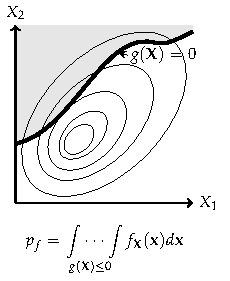
\includegraphics[width=.32\textwidth]{./figures/f-01-02-a-FORM}}
  \hfill
  \subfloat[][]{\label{fig:f-01-02-b}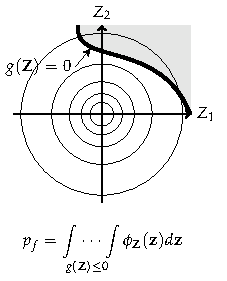
\includegraphics[width=.32\textwidth]{./figures/f-01-02-b-FORM}}
  \hfill
  \subfloat[][]{\label{fig:f-01-02-c}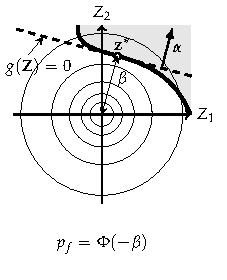
\includegraphics[width=.32\textwidth]{./figures/f-01-02-c-FORM}}
\caption[First Order Reliability Method]{First Order Reliability Method. (a) Representation of a physical space with a set $\mathbf{X}$ of any two random variables. The shaded area denotes the failure domain and $g(\mathbf{X})=0$ the failure surface. (b) After transformation in the normalized space, the random variables $\mathbf{Z}$ are now uncorrelated and standardized normally distributed, also the failure surface is transformed into $g(\mathbf{X})=0$. (c) FORM corresponds to a linearization of the failure surface $g(\mathbf{X})=0$. Performing this method, the design point $\mathbf{z}^*$ and the reliability index $\beta$ can be computed.}
  \label{fig:f-01-02-FORM}
\end{figure}

\subsection{Citations}
\label{sec:citations}

Academic work almost always builds upon the work of others, and it is appropriate, indeed essential, that you discuss the related and previous work of others in your thesis. However, this must be done according to the rules of acceptable use.

Much of the advice in the section on books will pertain to other sources as well. Their long history as a formal publication ensures, in particular, that the variations in author names and titles will serve as a model for constructing documentary notes and bibliography entries for many other types of sources.

The Chicago Manual of Style\footnote{\cite{chicago2010}}, implemented here in its 16th edition, has long, been one of the most influential style guides for writers and publishers. While one’s choices are now perhaps more extensive than ever, the Manual at least still provides a widely-recognized, and widely-utilized, standard.

A full reference must include enough information to enable an interested reader to locate the book. Most references contain at least some information not strictly needed for that purpose but potentially helpful nonetheless. The elements listed below are included, where applicable, in full documentary notes and bibliography entries.

%\begin{refsection}
The author appears as part of the narrative:
\begin{IMleftrightskip}
 \citet[p.100]{Nowak2000} show how to calculate the reliability index $\beta$, by using geometric properties.
\end{IMleftrightskip}

Otherwise, in parentheses:
\begin{IMleftrightskip}
A near linear relationship can be obtained between ultimate flexural and shear capacity of a RC section, if pitting corrosion occurs \citep{Stewart2009}.
\end{IMleftrightskip}
%\printbibliography[heading=none]
%\end{refsection}

% ===========================================================================
% EOF
%

%%% Local Variables:
%%% mode: latex
%%% TeX-master: "../main"
%%% End:
